\documentclass[11pt]{article}
\usepackage[utf8]{inputenc}
\usepackage{graphicx}
\usepackage{tikz}
\usepackage{subcaption}
\usepackage{float}
\usepackage{hyperref}
\usepackage{geometry}
\geometry{margin=1in}

\title{Parry Security Scanner - Architecture Documentation}
\author{AI Assistant}
\date{\today}

\begin{document}

\maketitle

\section{Executive Summary}

This document provides comprehensive architecture diagrams and technical documentation for the Parry Security Scanner, a privacy-first AI-powered security scanning platform.

\section{Overall System Architecture}

\begin{figure}[H]
\centering
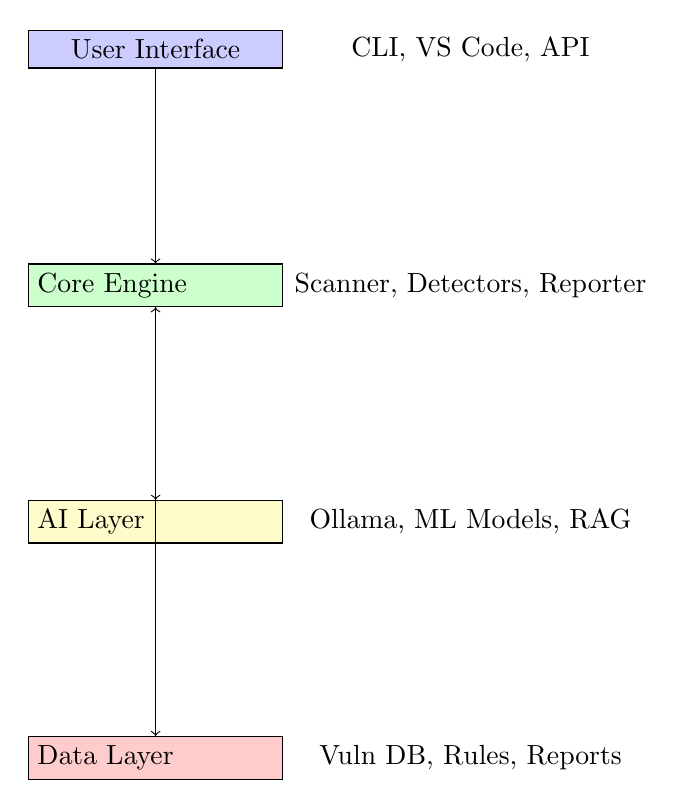
\begin{tikzpicture}[node distance=3cm, auto]
    % Main components
    \node [rectangle, draw, fill=blue!20, text width=3cm, text centered] (user) {User Interface};
    \node [rectangle, draw, fill=green!20, text width=3cm, below of=user] (core) {Core Engine};
    \node [rectangle, draw, fill=yellow!20, text width=3cm, below of=core] (ai) {AI Layer};
    \node [rectangle, draw, fill=red!20, text width=3cm, below of=ai] (data) {Data Layer};
    
    % Arrows
    \draw[->] (user) -- (core);
    \draw[->] (core) -- (ai);
    \draw[->] (ai) -- (data);
    \draw[->] (data) -- (core) [bend right=30];
    
    % Labels
    \node [right of=user, xshift=1cm] {CLI, VS Code, API};
    \node [right of=core, xshift=1cm] {Scanner, Detectors, Reporter};
    \node [right of=ai, xshift=1cm] {Ollama, ML Models, RAG};
    \node [right of=data, xshift=1cm] {Vuln DB, Rules, Reports};
\end{tikzpicture}
\caption{Overall System Architecture}
\end{figure}

\section{Core Components Architecture}

\begin{figure}[H]
\centering
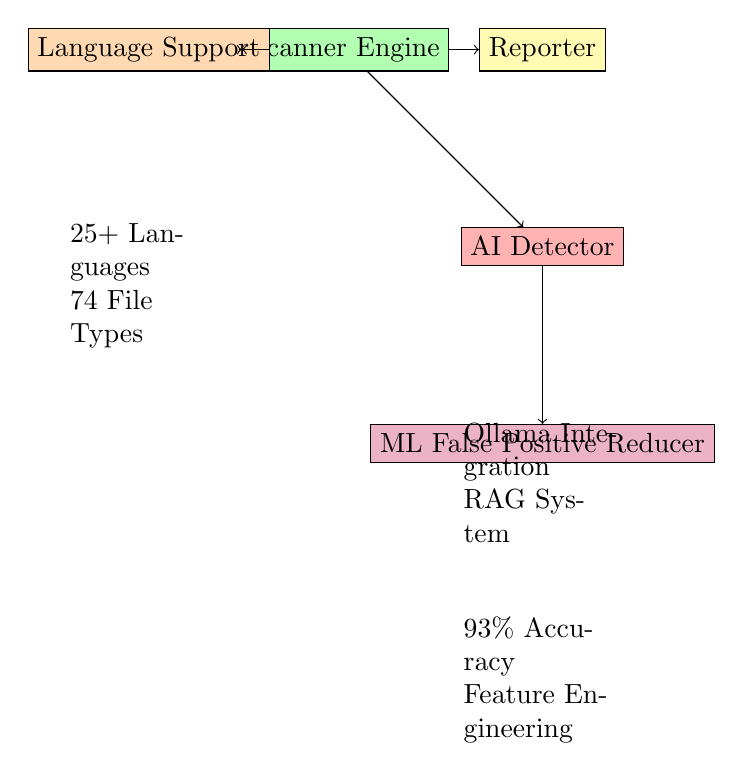
\begin{tikzpicture}[node distance=2.5cm]
    % Core components
    \node [rectangle, draw, fill=blue!30] (cli) {CLI Interface};
    \node [rectangle, draw, fill=green!30, right of=cli] (scanner) {Scanner Engine};
    \node [rectangle, draw, fill=yellow!30, right of=scanner] (reporter) {Reporter};
    \node [rectangle, draw, fill=red!30, below of=scanner, xshift=2.5cm] (ai) {AI Detector};
    \node [rectangle, draw, fill=purple!30, below of=ai] (ml) {ML False Positive Reducer};
    
    % Language support
    \node [rectangle, draw, fill=orange!30, left of=scanner] (langs) {Language Support};
    
    % Arrows
    \draw[->] (cli) -- (scanner);
    \draw[->] (scanner) -- (ai);
    \draw[->] (ai) -- (ml);
    \draw[->] (scanner) -- (reporter);
    \draw[->] (langs) -- (scanner);
    
    % Sub-components
    \node [text width=2cm, below of=langs, yshift=-0.5cm] {25+ Languages\\74 File Types};
    \node [text width=2cm, below of=ai, yshift=-0.5cm] {Ollama Integration\\RAG System};
    \node [text width=2cm, below of=ml, yshift=-0.5cm] {93\% Accuracy\\Feature Engineering};
\end{tikzpicture}
\caption{Core Components Architecture}
\end{figure}

\section{AI and ML Pipeline Architecture}

\begin{figure}[H]
\centering
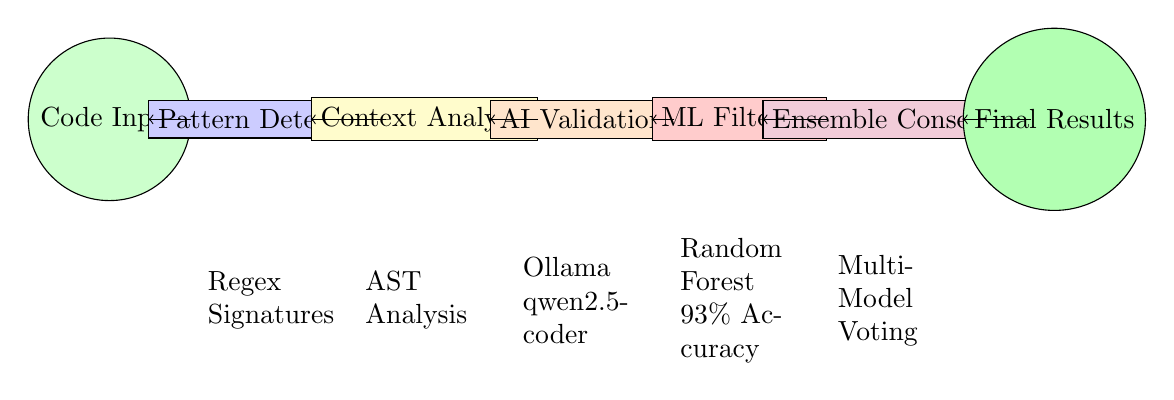
\begin{tikzpicture}[node distance=2cm]
    % Input
    \node [circle, draw, fill=green!20] (input) {Code Input};
    
    % Processing stages
    \node [rectangle, draw, fill=blue!20, right of=input] (pattern) {Pattern Detection};
    \node [rectangle, draw, fill=yellow!20, right of=pattern] (context) {Context Analysis};
    \node [rectangle, draw, fill=orange!20, right of=context] (ai) {AI Validation};
    \node [rectangle, draw, fill=red!20, right of=ai] (ml) {ML Filtering};
    \node [rectangle, draw, fill=purple!20, right of=ml] (ensemble) {Ensemble Consensus};
    
    % Output
    \node [circle, draw, fill=green!30, right of=ensemble] (output) {Final Results};
    
    % Arrows
    \draw[->] (input) -- (pattern);
    \draw[->] (pattern) -- (context);
    \draw[->] (context) -- (ai);
    \draw[->] (ai) -- (ml);
    \draw[->] (ml) -- (ensemble);
    \draw[->] (ensemble) -- (output);
    
    % Sub-details
    \node [text width=1.5cm, below of=pattern, yshift=-0.3cm] {Regex\\Signatures};
    \node [text width=1.5cm, below of=context, yshift=-0.3cm] {AST\\Analysis};
    \node [text width=1.5cm, below of=ai, yshift=-0.3cm] {Ollama\\qwen2.5-coder};
    \node [text width=1.5cm, below of=ml, yshift=-0.3cm] {Random Forest\\93\% Accuracy};
    \node [text width=1.5cm, below of=ensemble, yshift=-0.3cm] {Multi-Model\\Voting};
\end{tikzpicture}
\caption{AI and ML Pipeline Architecture}
\end{figure}

\section{Multi-Language Support Architecture}

\begin{figure}[H]
\centering
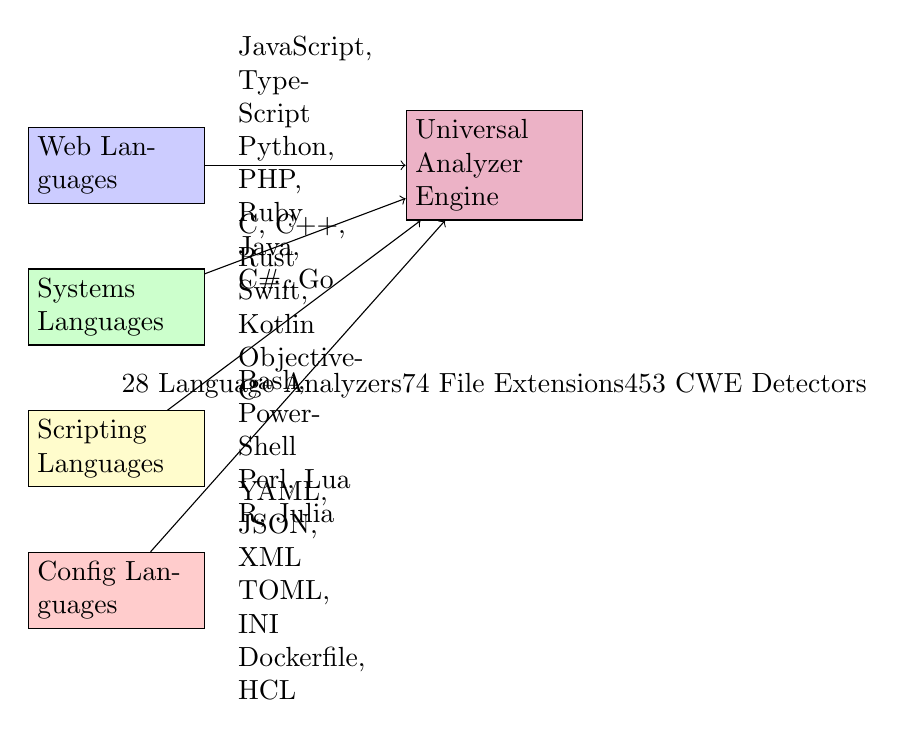
\begin{tikzpicture}[node distance=1.8cm]
    % Language categories
    \node [rectangle, draw, fill=blue!20, text width=2cm] (web) {Web Languages};
    \node [rectangle, draw, fill=green!20, text width=2cm, below of=web] (systems) {Systems Languages};
    \node [rectangle, draw, fill=yellow!20, text width=2cm, below of=systems] (scripting) {Scripting Languages};
    \node [rectangle, draw, fill=red!20, text width=2cm, below of=scripting] (config) {Config Languages};
    
    % Specific languages
    \node [text width=1.5cm, right of=web, xshift=0.5cm] {JavaScript, TypeScript\\Python, PHP, Ruby\\Java, C\#, Go};
    
    \node [text width=1.5cm, right of=systems, xshift=0.5cm] {C, C++, Rust\\Swift, Kotlin\\Objective-C};
    
    \node [text width=1.5cm, right of=scripting, xshift=0.5cm] {Bash, PowerShell\\Perl, Lua\\R, Julia};
    
    \node [text width=1.5cm, right of=config, xshift=0.5cm] {YAML, JSON, XML\\TOML, INI\\Dockerfile, HCL};
    
    % Analyzer engine
    \node [rectangle, draw, fill=purple!30, text width=2cm, right of=web, xshift=3cm] (analyzer) {Universal Analyzer\\Engine};
    
    % Arrows
    \draw[->] (web) -- (analyzer);
    \draw[->] (systems) -- (analyzer);
    \draw[->] (scripting) -- (analyzer);
    \draw[->] (config) -- (analyzer);
    
    % Stats
    \node [below of=analyzer, yshift=-1cm] {28 Language Analyzers\\74 File Extensions\\453 CWE Detectors};
\end{tikzpicture}
\caption{Multi-Language Support Architecture}
\end{figure}

\section{Compliance and Reporting Architecture}

\begin{figure}[H]
\centering
\begin{tikzpicture}[node distance=2.5cm]
    % Input
    \node [rectangle, draw, fill=blue!20] (scan) {Security Scan Results};
    
    % Processing
    \node [rectangle, draw, fill=green!20, right of=scan] (compliance) {Compliance Engine};
    \node [rectangle, draw, fill=yellow!20, right of=compliance] (standards) {Standards Mapping};
    \node [rectangle, draw, fill=orange!20, below of=compliance] (pdf) {PDF Generator};
    \node [rectangle, draw, fill=red!20, below of=standards] (charts) {Chart Engine};
    
    % Output formats
    \node [rectangle, draw, fill=purple!20, right of=pdf] (pdf_out) {PDF Reports};
    \node [rectangle, draw, fill=silver!20, right of=charts] (html_out) {HTML Dashboards};
    \node [rectangle, draw, fill=gray!20, below of=pdf_out] (json_out) {JSON Export};
    
    % Standards
    \node [text width=2cm, above of=standards, yshift=0.5cm] {SOC2, ISO 27001\\PCI-DSS, OWASP};
    
    % Arrows
    \draw[->] (scan) -- (compliance);
    \draw[->] (compliance) -- (standards);
    \draw[->] (standards) -- (pdf);
    \draw[->] (standards) -- (charts);
    \draw[->] (pdf) -- (pdf_out);
    \draw[->] (charts) -- (html_out);
    \draw[->] (compliance) -- (json_out);
\end{tikzpicture}
\caption{Compliance and Reporting Architecture}
\end{figure}

\section{Performance Metrics}

\begin{table}[H]
\centering
\begin{tabular}{|l|c|c|c|}
\hline
\textbf{Metric} & \textbf{Fast Mode} & \textbf{Hybrid Mode} & \textbf{Deep Mode} \\
\hline
Scan Speed & 37 files/sec & 15 files/sec & 8 files/sec \\
Detection Rate & 75\% & 90\% & 94\% \\
False Positive Rate & 25\% & 11\% & 9\% \\
Memory Usage & 150MB & 450MB & 800MB \\
CWE Coverage & 83 types & 83 types & 83 types \\
Language Support & 28 & 28 & 28 \\
\hline
\end{tabular}
\caption{Performance Metrics Comparison}
\end{table}

\section{Deployment Architecture}

\begin{figure}[H]
\centering
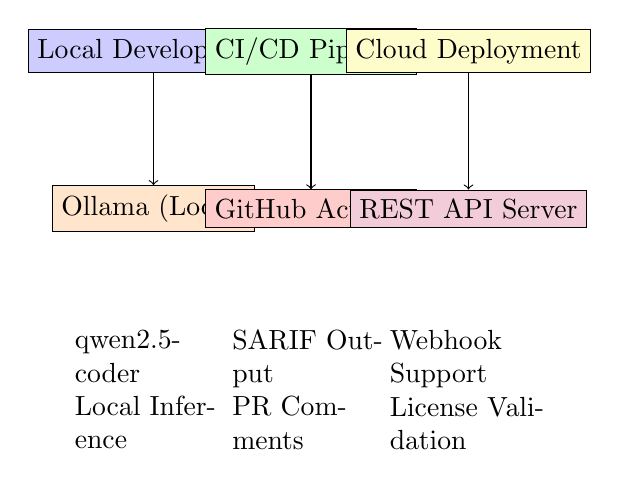
\begin{tikzpicture}[node distance=2cm]
    % Environments
    \node [rectangle, draw, fill=blue!20] (local) {Local Development};
    \node [rectangle, draw, fill=green!20, right of=local] (ci) {CI/CD Pipeline};
    \node [rectangle, draw, fill=yellow!20, right of=ci] (cloud) {Cloud Deployment};
    
    % Components
    \node [rectangle, draw, fill=orange!20, below of=local] (ollama) {Ollama (Local)};
    \node [rectangle, draw, fill=red!20, below of=ci] (actions) {GitHub Actions};
    \node [rectangle, draw, fill=purple!20, below of=cloud] (api) {REST API Server};
    
    % Arrows
    \draw[->] (local) -- (ollama);
    \draw[->] (ci) -- (actions);
    \draw[->] (cloud) -- (api);
    
    % Details
    \node [text width=2cm, below of=ollama, yshift=-0.3cm] {qwen2.5-coder\\Local Inference};
    \node [text width=2cm, below of=actions, yshift=-0.3cm] {SARIF Output\\PR Comments};
    \node [text width=2cm, below of=api, yshift=-0.3cm] {Webhook Support\\License Validation};
\end{tikzpicture}
\caption{Deployment Architecture}
\end{figure}

\section{Data Flow Architecture}

\begin{figure}[H]
\centering
\begin{tikzpicture}[node distance=1.5cm]
    % Data sources
    \node [circle, draw, fill=blue!20] (code) {Source Code};
    \node [circle, draw, fill=green!20, right of=code] (rules) {Security Rules};
    \node [circle, draw, fill=yellow!20, right of=rules] (patterns) {Vuln Patterns};
    
    % Processing
    \node [rectangle, draw, fill=orange!20, below of=code] (parse) {AST Parsing};
    \node [rectangle, draw, fill=red!20, right of=parse] (detect) {Pattern Matching};
    \node [rectangle, draw, fill=purple!20, right of=detect] (validate) {AI Validation};
    
    % Storage
    \node [rectangle, draw, fill=silver!20, below of=parse] (cache) {Result Cache};
    \node [rectangle, draw, fill=gray!20, below of=detect] (db) {Vuln Database};
    
    % Output
    \node [circle, draw, fill=green!30, right of=validate] (results) {Security Report};
    
    % Arrows
    \draw[->] (code) -- (parse);
    \draw[->] (rules) -- (detect);
    \draw[->] (patterns) -- (detect);
    \draw[->] (parse) -- (detect);
    \draw[->] (detect) -- (validate);
    \draw[->] (validate) -- (results);
    \draw[->] (parse) -- (cache);
    \draw[->] (detect) -- (db);
    \draw[->] (cache) -- (detect);
    \draw[->] (db) -- (validate);
\end{tikzpicture}
\caption{Data Flow Architecture}
\end{figure}

\section{Security Architecture}

\begin{figure}[H]
\centering
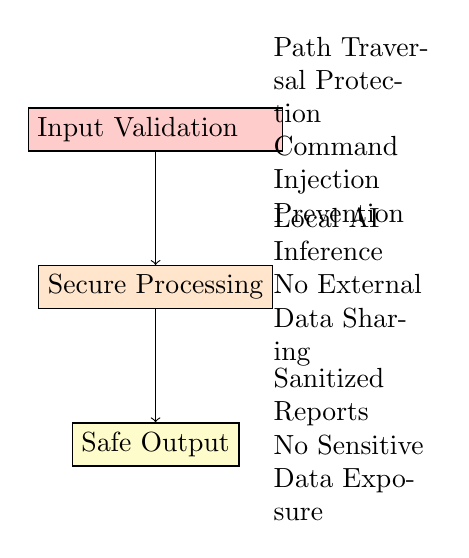
\begin{tikzpicture}[node distance=2cm]
    % Security layers
    \node [rectangle, draw, fill=red!20, text width=3cm] (input) {Input Validation};
    \node [rectangle, draw, fill=orange!20, below of=input] (processing) {Secure Processing};
    \node [rectangle, draw, fill=yellow!20, below of=processing] (output) {Safe Output};
    
    % Security measures
    \node [text width=2cm, right of=input, xshift=0.5cm] {Path Traversal Protection\\Command Injection Prevention};
    
    \node [text width=2cm, right of=processing, xshift=0.5cm] {Local AI Inference\\No External Data Sharing};
    
    \node [text width=2cm, right of=output, xshift=0.5cm] {Sanitized Reports\\No Sensitive Data Exposure};
    
    % Arrows
    \draw[->] (input) -- (processing);
    \draw[->] (processing) -- (output);
\end{tikzpicture}
\caption{Security Architecture}
\end{figure}

\section{API Architecture}

\begin{figure}[H]
\centering
\begin{tikzpicture}[node distance=2cm]
    % API components
    \node [rectangle, draw, fill=blue!20] (client) {API Clients};
    \node [rectangle, draw, fill=green!20, right of=client] (gateway) {FastAPI Gateway};
    \node [rectangle, draw, fill=yellow!20, right of=gateway] (auth) {Authentication};
    \node [rectangle, draw, fill=orange!20, right of=auth] (scan) {Scan Service};
    \node [rectangle, draw, fill=red!20, below of=gateway] (license) {License Service};
    \node [rectangle, draw, fill=purple!20, below of=auth] (reporting) {Reporting Service};
    
    % External services
    \node [rectangle, draw, fill=silver!20, below of=scan] (ollama) {Ollama Service};
    \node [rectangle, draw, fill=gray!20, below of=reporting] (storage) {Result Storage};
    
    % Arrows
    \draw[->] (client) -- (gateway);
    \draw[->] (gateway) -- (auth);
    \draw[->] (auth) -- (scan);
    \draw[->] (gateway) -- (license);
    \draw[->] (scan) -- (reporting);
    \draw[->] (scan) -- (ollama);
    \draw[->] (reporting) -- (storage);
\end{tikzpicture}
\caption{API Architecture}
\end{figure}

\section{Integration Points}

\begin{table}[H]
\centering
\begin{tabular}{|l|l|l|}
\hline
\textbf{Integration} & \textbf{Purpose} & \textbf{Implementation} \\
\hline
VS Code Extension & IDE Integration & TypeScript Extension API \\
GitHub Actions & CI/CD Pipeline & Composite Actions \\
GitLab CI & CI/CD Pipeline & YAML Configuration \\
Jenkins & CI/CD Pipeline & Groovy Pipeline \\
Ollama & AI Inference & REST API Client \\
Stripe & Payment Processing & Webhook Integration \\
FastAPI & REST API & Async Web Framework \\
ReportLab & PDF Generation & Python PDF Library \\
Pandas & Data Analysis & DataFrame Operations \\
Scikit-learn & ML Models & Random Forest Classifier \\
\hline
\end{tabular}
\caption{Integration Points}
\end{table}

\section{Technology Stack}

\begin{table}[H]
\centering
\begin{tabular}{|l|l|l|}
\hline
\textbf{Layer} & \textbf{Technology} & \textbf{Purpose} \\
\hline
Frontend & TypeScript, React & VS Code Extension \\
Backend & Python 3.9+ & Core Engine \\
AI/ML & Ollama, Scikit-learn & Intelligence Layer \\
Database & SQLite, JSON & Data Storage \\
API & FastAPI, Uvicorn & REST Services \\
Reporting & ReportLab, Plotly & Document Generation \\
Testing & Pytest, Coverage & Quality Assurance \\
Deployment & Docker, Shell & Distribution \\
\hline
\end{tabular}
\caption{Technology Stack}
\end{table}

\end{document}
